\chapter{Methodology}\label{sec:Methodology}

\section{Battery Model}\label{BatteryModel}
% Section 1 — Battery Modelling
The Battery Management System (\acs{BMS}) is responsible for calculating estimates of critical internal variables, such as 
the State of Charge (\acs{SOC}) and State of Health (\acs{SOH}). Consequently, implementing a high-fidelity mathematical framework
that captures the complex dynamics of the battery is essential. A widely adopted approach is the equivalent-circuit model (\acs{ECM}),
in which the behaviour of a lithium-ion cell is represented as an electrical circuit. Such model requires the characterisation 
of specific parameters and cell dynamics through conducted tests under controlled conditions~\cite{plett2015battery}.

\begin{figure}[H]
    \centering
    \begin{circuitikz}[american]
        \draw
        % Start with the voltage source
        (0,0) to[battery2, invert, l=$OCV(z)$] (0,3)
        
        % Series resistor R0
        to[R, l=$R_0$, i<=$I$] (3,3)
        
        % First RC parallel block
        -- (3,3.5) to[R, l=$R_1$] (5,3.5) -- (5,3)
        (3,3) -- (3,2.5) to[C, l_=$C_1$] (5,2.5) -- (5,3)
        
        % Second RC parallel block
        (5,3) -- (5,3.5) to[R, l=$R_2$] (7,3.5) -- (7,3) % Changed R1 to R2 to match your equations
        (5,3) -- (5,2.5) to[C, l_=$C_2$] (7,2.5) -- (7,3)
        
        % Connection to output terminals
        (7,3) to[short, -o] (8,3) node[right] {$+$}
        (0,0) to[short, -o] (8,0) node[right] {$-$}
        
        % Label for total voltage U
        (8,1.5) node {$y_k$};
    \end{circuitikz}
    \caption{Second-order Thévenin equivalent circuit model.}
    \label{img:2oTECM} 
\end{figure}

The discrete-time \acs{ECM} used in this study is defined by three primary components: the State of Charge, the diffusion 
currents within the RC branches, and the hysteresis voltage.

The State of Charge at a discrete-time index $k$, denoted as $z_k$, represents the ratio of the remaining 
capacity to the nominal capacity of the cell. Its temporal evolution is governed by the following relationship:
\begin{equation}
    z_{k+1} = z_k - \eta \frac{\Delta t}{Q}(i_k + w_k)
    \label{eq:zESC}
\end{equation}

For this study, the battery is represented as a second-order Thévenin equivalent circuit, as shown in 
Figure~\ref{img:2oTECM}. The polarisation and diffusion effects are modelled using 
two resistor-capacitor networks. The currents circulating through the resistors $R_1$ and $R_2$ at 
time step $k$ are denoted as $i_{R1,k}$ and $i_{R2,k}$ respectively, and their discrete-time evolution is described by:


\begin{equation}
    i_{R1_{k+1}} = \tau_1 i_{R1_{k}} + (1 - \tau_1)(i_k + w_k)
    \label{eq:iR1}
\end{equation}

\begin{equation}
    i_{R2_{k+1}} = \tau_2 i_{R2_{k}} + (1 - \tau_2)(i_k + w_k)
    \label{eq:iR2}
\end{equation}

Where the time constants $\tau_1$ and $\tau_2$ are defined as:

\begin{equation}
    \tau_1 = e^{-\frac{\Delta t}{(R_1 C_1)}}
    \label{eq:tau1}
\end{equation}

\begin{equation}
    \tau_2 = e^{-\frac{\Delta t}{(R_2 C_2)}}
    \label{eq:tau2}
\end{equation}

The third component is the hysteresis state $h_k$. The discrete-time evolution of the hysteresis state is modelled as:
\begin{equation}
    h_{k+1} = e^{\left(-\left| \frac{\eta_k i_k \gamma \Delta t}{Q} \right|\right)} h_k + 
    (e^{\left(-\left| \frac{\eta_k i_k \gamma \Delta t}{Q} \right|\right)} -1) \text{sgn}(i_k)
    \end{equation}

In this work, the hysteresis state is excluded. Under the specific operating conditions considered for this application, 
hysteresis effects are small, and omitting this state reduces the computational complexity of the model without incurring a 
significant loss in estimation accuracy.

Finally, the terminal output voltage $y_k$ is defined by the following observation equation:

\begin{equation}
    y_k = OCV(z_k) - R_1 i_{R1_{k}} - R_2 i_{R2_{k}} - R_0 i_k + v_k
    \label{eq:y_kESC}
\end{equation}

$z_k$ is the state of charge for time $k$.\\
$i_k$ is the current exchanged by the battery at its connection in [A].\\
$i_{R1_{k+1}}$ is the current through the resistance 1 for the time $k$ in [A].\\
$i_{R2_{k+1}}$ is the current through the resistance 2 for the time $k$ in [A].\\
$y_k$ is the voltage across the terminals of the battery for the time k in [V].\\
$\eta$ is the Coulombic efficiency.\\
$\Delta t$ is the time step.\\
$R_0$ is the pure ohmic internal resistance of the battery in [$\Omega$].\\
$R_1$ and $R_2$ are the resistance for the RC block 1 and 2 in [$\Omega$].\\
$C_1$ and $C_2$ are the capacitance for the RC block 1 and 2 in [F].\\
$OCV(z_k)$ is the Open Circuit Voltage corresponding to the state of charge $z_k$ in [V].\\
$Q$ is the Electric capacity in [As].

\subsection{Racing Motorcycle Battery Model}

The experimental methodology of this work focuses on the battery used to power the electric racing motorcycle developed at ETSEIB. 
The specific cell model used is the WeLion SHP270--30~\cite{welion2026shp270}, a type of Nickel Manganese Cobalt (\acs{NMC}) 
lithium-ion pouch cell with a nominal capacity of $30$ Ah and a nominal energy of $111$ Wh.~\acs{NMC} cells are typically 
used in high-performance racing applications due to their high energy density and favourable energy-to-weight ratio, 
as well as in electric vehicles~\cite{HassanTantaNMC}.
This cell was selected for both the experimental characterisation and the implementation of the estimation algorithms.

\section{OCV-SOC Curve Characterisation}\label{OCVSOC}

The \acs{OCV}-\acs{SOC} curve describes the relationship between the \ac{OCV} and the \ac{SOC} of the cell. 
This relationship is a key element of the battery model described in Section~\ref{BatteryModel}, since it is necessary for the 
output equation~\eqref{eq:y_kESC} and to compute the differential term $dOCV/dz$ used in the \ac{EKF} implementation 
shown in Section~\ref{Kalman}.

Three separate experimental tests are required to obtain the \ac{OCV}-\ac{SOC} curve. Through the first two tests, 
described in Sections~\ref{DischargeTest} and~\ref{ChargeTest}, the cell capacity, exchanged energy, and efficiency are computed. 
For all three tests, the terminal voltage, current and time 
must be continuously recorded using a power analyser. The tests are as follows:

\begin{figure}[H]
    \centering
    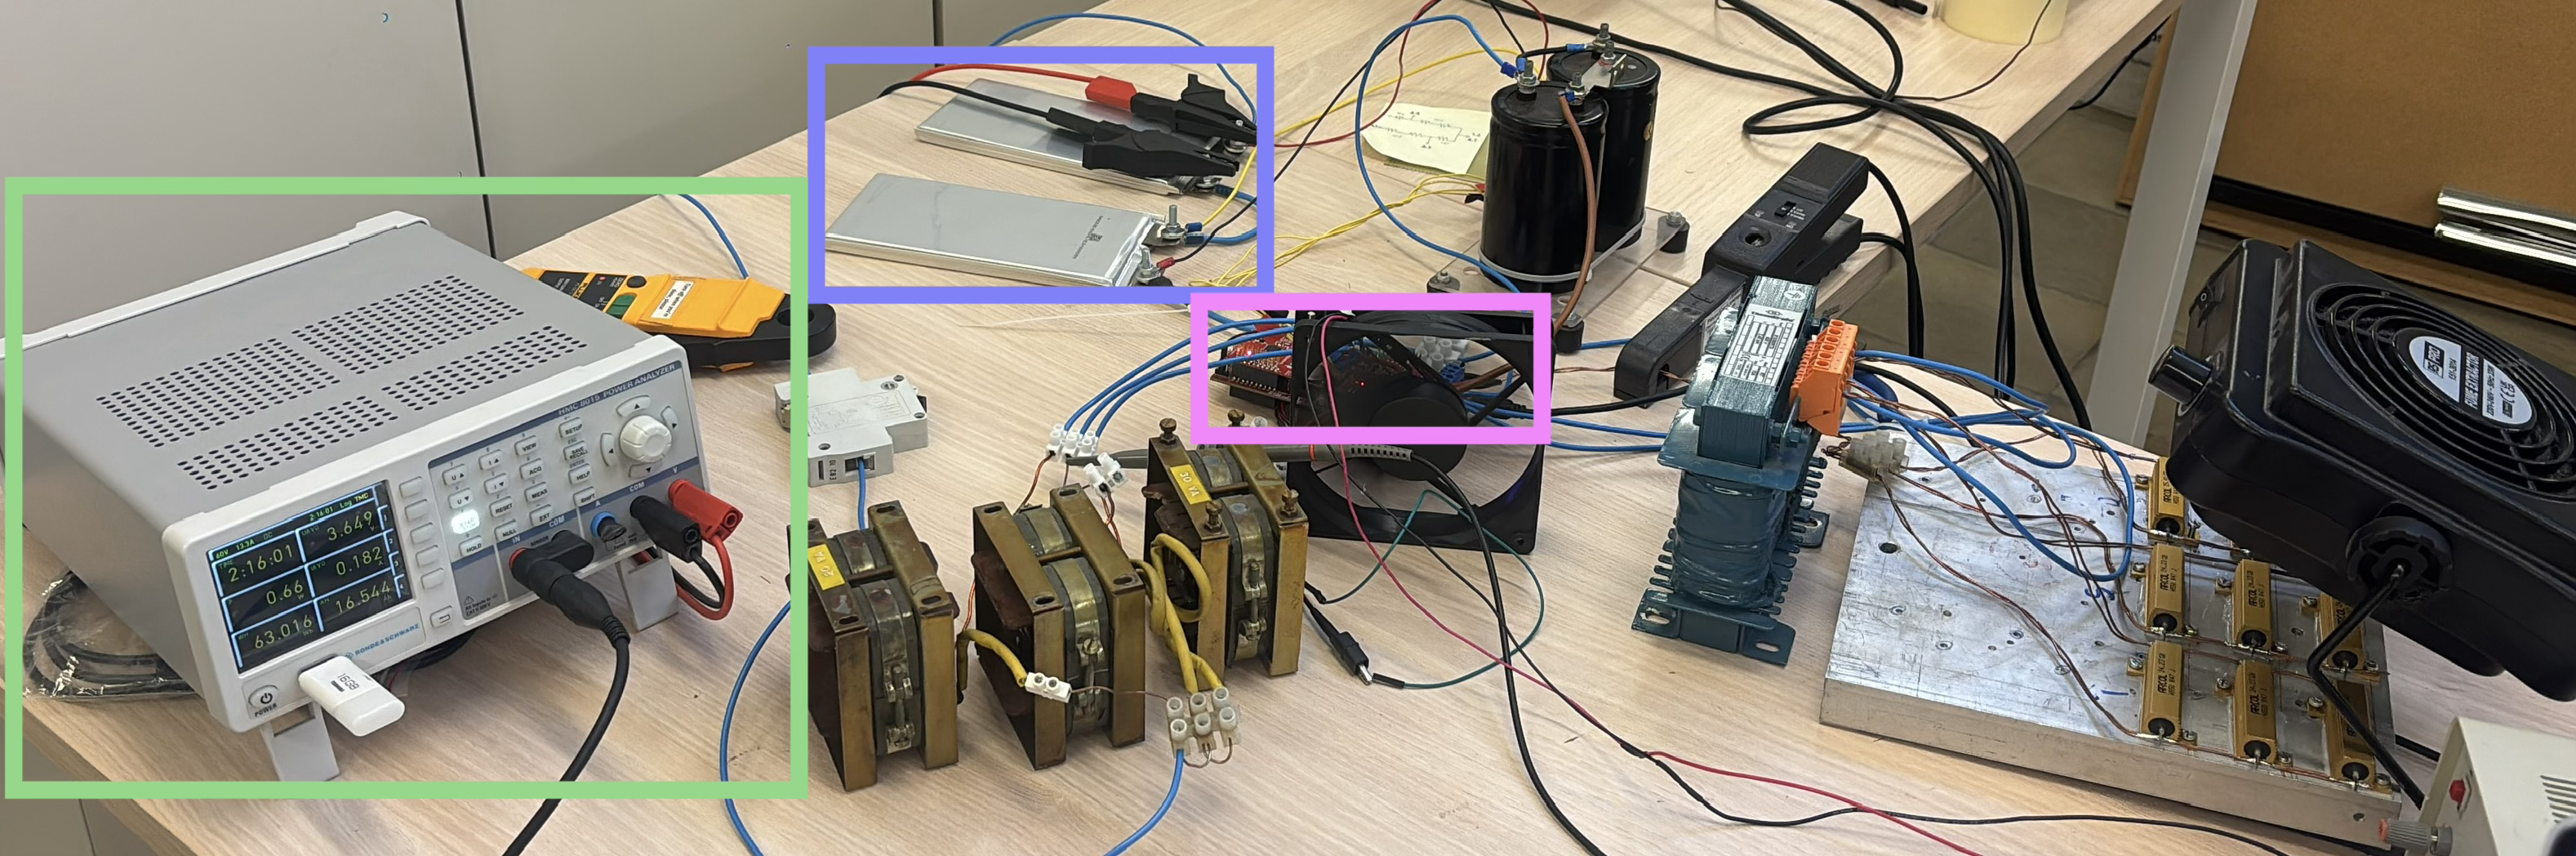
\includegraphics[width = 1\textwidth]{Images/Test_Setup.png}
    \caption{Battery test setup, power analyzer(green), batteries (lilac), and National Instruments microcontroller (pink).}
    \label{Testsetup}
\end{figure}

\subsection{Discharge Test}\label{DischargeTest}

The discharge test must be conducted at a low constant current to minimise internal resistance losses, 
ensuring the capacity measurement accurately reflects the true electrochemical capacity of the cell. 
Due to the safety risks inherent to handling \ac{Li-ion} batteries, the test requires continuous laboratory supervision. 
Consequently, the magnitude of the discharge current is constrained by the maximum safe operating window and the 
nominal capacity of the cell under test. This operational boundary is established as follows:

\begin{equation}
    I_{dis} \le \frac{Q_{nom}}{t_{dis}}
\end{equation}

\noindent where $Q_{nom}$ represents the nominal capacity of the cell and $t_{dis}$ is the maximum permissible 
duration for continuous supervision. Based on this constraint, a conservative constant discharge current $I_{dis}$ 
is selected to guarantee the test concludes within the monitored timeframe. 

From the recorded current profile and the total discharge duration $t_{dis}$, the actual discharge capacity 
of the cell $Q$ is determined by,

\begin{equation}
    Q = I_{dis} t_{dis}
    \label{eq:ActualCapacity}
\end{equation}

The total energy released by the cell during the discharge process is theoretically defined by integrating the 
instantaneous power over the total test duration as,

\begin{equation}
    E_{dis} = \int_{0}^{t_{dis}} v(t)\, i(t) \, dt
    \label{eq:Edis}
\end{equation}

In practice, because data collection relies on discrete time sampling, the total energy is calculated numerically. 
Assuming a constant sampling interval $\Delta t$, the discrete energy calculation is expressed as:

\begin{equation}
    E_{dis} = \sum_{n=1}^{N} v_n i_n \Delta t
    \label{eq:EdisDiscrete}
\end{equation}

\noindent Where the parameters from equations~\ref{eq:ActualCapacity},~\ref{eq:Edis}, and~\ref{eq:EdisDiscrete} are 
defined as follows,

\begin{description}
    \item[$Q$] Actual discharge capacity of the cell [Ah].
    \item[$I_{dis}$] Constant discharge current magnitude [A].
    \item[$t_{dis}$] Total duration of the discharge test [h].
    \item[$E_{dis}$] Total energy released during discharge [Wh].
    \item[$v(t), v_n$] Continuous and discrete measured terminal voltage [V].
    \item[$i(t), i_n$] Continuous and discrete measured discharge current [A].
    \item[$\Delta t$] Sampling time step expressed in hours.
    \item[$N$] Total number of recorded data samples.
\end{description}

\subsection{Charge Test}\label{ChargeTest}
In contrast to the discharge test, the charging procedure does not maintain a single constant current throughout its duration. 
Instead, it follows a standard \ac{CC-CV} protocol, which is critical for safely maximising 
the \ac{SOC} without exceeding the cell's upper voltage limit. This behaviour is illustrated in Figure~\ref{fig:cccv_profile}.

\begin{figure}[H]
    \centering
    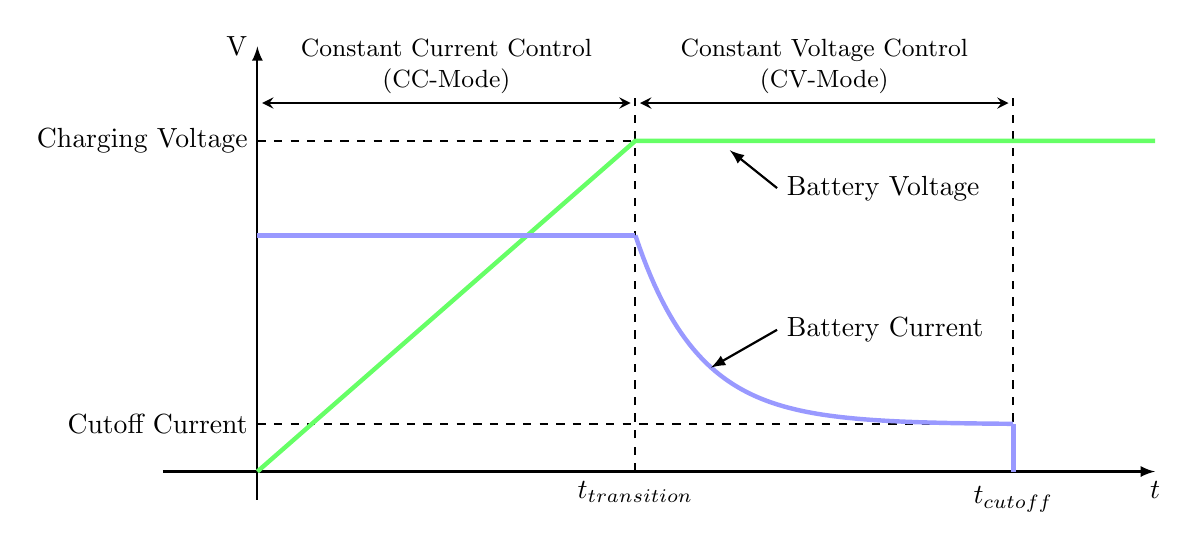
\begin{tikzpicture}[>=latex, scale=1.2]
        
        % Coordinates for alignment
        \def\xtrans{4.0}  % Time where CC switches to CV
        \def\xcutoff{8.0} % Cutoff time
        \def\xmax{9.5}    % Max X axis
        \def\ymax{4.5}    % Max Y axis
        \def\vchg{3.5}    % Charging voltage level
        \def\icurr{2.5}   % Constant current level
        \def\icut{0.5}    % Cutoff current level

        % --- Axes ---
        \draw[->, thick] (-1,0) -- (\xmax,0) node[below] {$t$};
        \draw[->, thick] (0,-0.3) -- (0,\ymax) node[left] {V};

        % --- Dashed reference lines ---
        \draw[dashed, thick] (0,\vchg) -- (\xtrans,\vchg);
        \draw[dashed, thick] (0,\icut) -- (\xcutoff,\icut);
        \draw[dashed, thick] (\xtrans,0) -- (\xtrans,\vchg + 0.5);
        \draw[dashed, thick] (\xcutoff,0) -- (\xcutoff,\vchg + 0.5);

        % --- Y-Axis Labels ---
        \node[left] at (0,\vchg) {Charging Voltage};
        \node[left] at (0,\icut) {Cutoff Current};
        
        % --- X-Axis Labels ---
        \node[below] at (\xtrans,0) {$t_{\text{transition}}$};
        \node[below, yshift=-2pt] at (\xcutoff,0) {$t_{\text{cutoff}}$};

        % --- Curves ---
        % Battery Voltage (Red)
        \draw[ultra thick, green!60] (0,0) -- (\xtrans,\vchg) -- (\xmax,\vchg);
        
        % Battery Current (Blue)
        \draw[ultra thick, blue!40] (0,\icurr) -- (\xtrans,\icurr);
        % Exponential decay curve from transition to cutoff
        \draw[ultra thick, blue!40] plot[domain=\xtrans:\xcutoff, samples=100] 
            (\x, {\icut + (\icurr-\icut)*exp(-1.5*(\x-\xtrans))});
        % Drop to zero at cutoff time
        \draw[ultra thick, blue!40] (\xcutoff,\icut) -- (\xcutoff,0);

        % --- Control Mode Labels & Green Arrows ---
        % CC Mode
        \draw[<->, >=stealth, thick, black] (0.05,\vchg + 0.4) -- (\xtrans-0.05,\vchg + 0.4);
        \node[above, align=center, font=\small] at (\xtrans/2, \vchg + 0.4) {Constant Current Control\\(CC-Mode)};

        % CV Mode
        \draw[<->, >=stealth, thick, black] (\xtrans+0.05,\vchg + 0.4) -- (\xcutoff-0.05,\vchg + 0.4);
        \node[above, align=center, font=\small] at ({(\xtrans+\xcutoff)/2}, \vchg + 0.4) {Constant Voltage Control\\(CV-Mode)};

        % --- Curve Labels and Pointers ---
        % Battery Voltage label
        \draw[->, thick] (\xtrans+1.5, \vchg-0.5) -- (\xtrans+1.0, \vchg-0.1);
        \node[right] at (\xtrans+1.5, \vchg-0.5) {Battery Voltage};

        % Battery Current label
        \draw[->, thick] (\xtrans+1.5, \icut+1.0) -- (\xtrans+0.8, \icut+0.6);
        \node[right] at (\xtrans+1.5, \icut+1.0) {Battery Current};

    \end{tikzpicture}
    \caption{Generic \ac{CC-CV} charging profile characterisation curve~\cite{CCCVcurve}.\protect\footnotemark}
    \label{fig:cccv_profile}
\end{figure}
\footnotetext{During the preparation of this work,
the author used Gemini 3.5 to produce Figure~\ref{fig:cccv_profile}. After using this tool, the author reviewed and
edited the content as necessary, and she assumes full responsibility for the content of the publication.}

During the constant current mode, a steady current pushes energy into the cell, causing the terminal voltage to rise linearly. 
Once the cell reaches its upper charging threshold, the control system switches to constant voltage mode; the voltage is clamped, 
and the current exponentially decays. The total energy consumed by the cell during this charging sequence ($E_{charge}$) 
is computed by integrating the continuous power profile:

\begin{equation}
    E_{charge} = \int_{0}^{t_{charge}} v(t)\, i(t) \, dt
    \label{eq:Echarge}
\end{equation}

Mirroring the discrete formulation used in the discharge analysis, 
the practical computation from experimental dataset values is computed as:

\begin{equation}
    E_{charge} = \sum_{n=1}^{M} v_n i_n \Delta t
    \label{eq:EchargeDiscrete}
\end{equation}

\noindent where $M$ represents the total number of sampling points accumulated across both charging phases. 
With both experimental energy parameters quantified, the net energy efficiency ($\eta$) of the battery system 
is calculated as,

\begin{equation}
    \eta = \frac{E_{dis}}{E_{charge}}
\end{equation}

\subsection{Pulses Test}\label{PulsesTest}
Characterising the \ac{OCV} vs. \ac{SOC} relationship requires executing an 
intermittent pulse discharge test. This profile applies consecutive, discrete discharge pulses designed 
to deplete the cell capacity by a precise, predetermined percentage step.

Each active current pulse is followed by an extended relaxation period, allowing the internal chemical 
diffusion transients to decay and the terminal voltage to stabilise to its true equilibrium OCV state. 
Using the actual capacity $Q$ obtained from the continuous discharge test (Section~\ref{DischargeTest}), 
the capacity step required for each specific depth of discharge interval, $Q_{step}$ is expressed by:

\begin{equation}
    Q_{step} = Q p_{step}
\end{equation}

\begin{equation}
    t_{dis_{5\%}} = \frac{Q_{5\%}}{I_{cons}}60
\end{equation}

\noindent where $p_{step}$ represents the chosen fractional capacity drop per pulse. 
To implement this configuration in the cycler software under a chosen constant test current ($I_{cons}$), 
the required active pulse duration ($t_{pulse}$) in minutes is calculated as:

\begin{equation}
    t_{pulse} = \frac{Q_{step}}{I_{cons}} 60
\end{equation}

\noindent where $t_{pulse}$ represents the explicit window length in minutes during which the current $I_{cons}$ 
must be drawn to accurately shift the cell down the \ac{SOC} tracking curve by the designated interval.

The sequential current profile configuration utilised to execute this experimental pulse sequence is illustrated 
schematically in Figure~\ref{fig:PulsesTest}.

\begin{figure}[H]
    \centering
    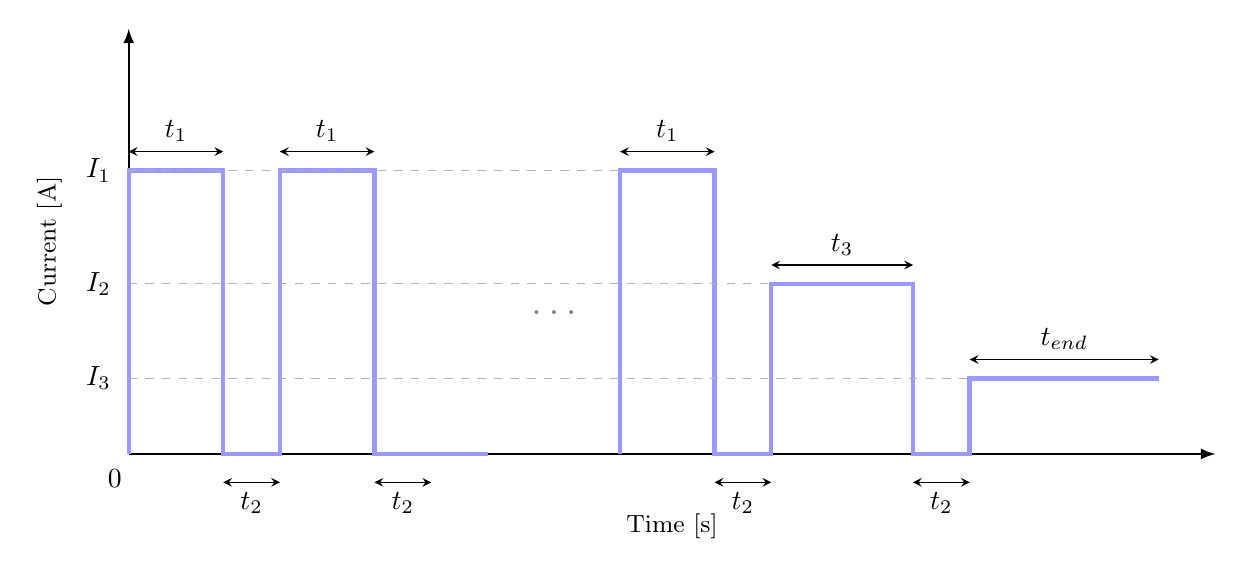
\begin{tikzpicture}[>=latex, scale=1.2]
        
        % --- Coordinates and Dimensions ---
        \def\xmax{11.5}    % Max X axis length
        \def\ymax{4.5}     % Max Y axis length
        
        \def\hIone{3.0}    % Height for I1
        \def\hItwo{1.8}    % Height for I2
        \def\hIthree{0.8}  % Height for I3
        \def\hRest{0.0}    % Height for Rest (0 A)

        % --- Axes (Starting exactly at 0,0) ---
        \draw[->, thick] (0,0) -- (\xmax,0);
        \draw[->, thick] (0,0) -- (0,\ymax);

        % --- Centered Axis Labels ---
        \node[below=18pt, font=\small] at (\xmax/2, 0) {Time [s]};
        % Increased above padding from 22pt to 35pt to push it safely left of the variables
        \node[rotate=90, above=7pt, font=\small] at (-0.4, \ymax/2) {Current [A]};

        % --- Y-Axis Variable Labels ---
        \node[left=3pt] at (0,\hIone) {$I_1$};
        \node[left=3pt] at (0,\hItwo) {$I_2$};
        \node[left=3pt] at (0,\hIthree) {$I_3$};
        \node[left=5pt, below=2pt] at (0,0) {0};

        % --- Profile Drawing (blue!40) ---
        \draw[ultra thick, blue!40] 
            (0,0) -- 
            (0,\hIone) -- (1.0,\hIone) -- 
            (1.0,\hRest) -- (1.6,\hRest) -- 
            (1.6,\hIone) -- (2.6,\hIone) -- 
            (2.6,\hRest) -- (3.2,\hRest) --
            (3.8,\hRest);
            
        % The Break Ellipsis (...)
        \node[gray, font=\bfseries\Large] at (4.5, 1.5) {$\dots$};
        
        \draw[ultra thick, blue!40]
            (5.2,\hRest) -- 
            (5.2,\hIone) -- (6.2,\hIone) -- 
            (6.2,\hRest) -- (6.8,\hRest) -- 
            % Intermediate pulse (I2)
            (6.8,\hItwo) -- (8.3,\hItwo) -- 
            (8.3,\hRest) -- (8.9,\hRest) -- 
            % Final continuous discharge (I3)
            (8.9,\hIthree) -- (10.9,\hIthree);

        % --- Dashed Reference Guidelines ---
        \draw[dashed, gray!60, thin] (0,\hIone) -- (5.2,\hIone);
        \draw[dashed, gray!60, thin] (0,\hItwo) -- (6.8,\hItwo);
        \draw[dashed, gray!60, thin] (0,\hIthree) -- (8.9,\hIthree);

        % --- Width Indicators (Arrows and Labels) ---
        % t1 active pulse widths
        \draw[<->, >=stealth, thin, black] (0, \hIone + 0.2) -- (1.0, \hIone + 0.2) node[midway, above] {$t_1$};
        \draw[<->, >=stealth, thin, black] (1.6, \hIone + 0.2) -- (2.6, \hIone + 0.2) node[midway, above] {$t_1$};
        \draw[<->, >=stealth, thin, black] (5.2, \hIone + 0.2) -- (6.2, \hIone + 0.2) node[midway, above] {$t_1$};
        
        % t3 active pulse width
        \draw[<->, >=stealth, thin, black] (6.8, \hItwo + 0.2) -- (8.3, \hItwo + 0.2) node[midway, above] {$t_3$};
        
        % tend active pulse width
        \draw[<->, >=stealth, thin, black] (8.9, \hIthree + 0.2) -- (10.9, \hIthree + 0.2) node[midway, above] {$t_{\text{end}}$};

        % t2 rest period widths (placed below the x-axis line)
        \draw[<->, >=stealth, thin, black] (1.0, -0.3) -- (1.6, -0.3) node[midway, below] {$t_2$};
        \draw[<->, >=stealth, thin, black] (2.6, -0.3) -- (3.2, -0.3) node[midway, below] {$t_2$};
        \draw[<->, >=stealth, thin, black] (6.2, -0.3) -- (6.8, -0.3) node[midway, below] {$t_2$};
        \draw[<->, >=stealth, thin, black] (8.3, -0.3) -- (8.9, -0.3) node[midway, below] {$t_2$};

    \end{tikzpicture}
    \caption{Representation of the current pulses.\protect\footnotemark}
    \label{fig:PulsesTest}
\end{figure}
\footnotetext{During the preparation of this work,
the author used Gemini 3.5 to produce Figure~\ref{fig:PulsesTest}. After using this tool, the author reviewed and
edited the content as necessary, and she assumes full responsibility for the content of the publication.}

As shown in the profile, the core characterisation routine consists of discrete active discharge periods of 
magnitude $I_1$ applied for a strict calculated duration $t_1$. Each individual current interaction is followed by 
an invariant relaxation period $t_2$ at zero current input $0\text{ A}$.

To accommodate changing operational bounds as the battery nears empty \ac{SOC} states, 
the profile incorporates an intermediate parameter stage featuring an altered current step 
magnitude $I_2$ maintained across an altered duration window $t_3$.

Finally, the total diagnostic routine transitions into a continuous constant-current 
depleted phase of magnitude $I_3$ for a remaining duration $t_{\text{end}}$, 
ensuring the battery system safely reaches its terminal lower voltage cut-off boundary.

\section{Parameter Identification}\label{Parameters}
% Section 2 — Parameter Identification

The accuracy of the \acs{ECM} is critically dependent on the precise identification of its internal parameters.
As described in Section~\ref{BatteryModel}, a 
second-order Thévenin equivalent circuit was selected for this work, therefore, the parameters to be identified are  
the Open Circuit Voltage, the Ohmic resistance $R_0$, and the resistances and capacitances 
of the two RC branches, $R_1$, $C_1$, $R_2$, and $C_2$.
\\
The conventional approach to parameter identification is the least-squares curve fitting of experimental voltage 
responses obtained during controlled charge and discharge cycles. 
A fundamental assumption of this method is that each test starts from zero initial conditions, which requires a
rest period of 30 minutes between tests~\cite{DEVARAKONDA2014}, making the full characterisation of a battery a time-consuming and 
impractical process.
\\
To overcome this limitation, the algebraic parameter identification method proposed by Devarakonda and Hu~\cite{DEVARAKONDA2014} 
is followed in this work. The key contribution of this method is that it extracts all circuit parameters simultaneously 
with the unknown initial conditions of the capacitor voltages, thereby eliminating the requirement for 
relaxation periods between tests and accelerating the characterisation process.
\\
The process can be divided into four stages, which will be described in Section~\ref{Teststeps}.

\subsection{Parameter Identification - Test Setup}
The setup for the parameter identification requires an electronic load (as in Figure~\ref{img:2oTECM_withLoad}) 
to draw a step discharge current $I$ which
will change to $I_1$ (as described in~\eqref{eq:step_current}) and the terminal voltage $v(t)$ to be recorded continuously. 

\begin{figure}[H]
    \centering
    \begin{circuitikz}[american]
        \draw
        % Start with the voltage source
        (0,0) to[battery2, invert, l=$OCV(z)$] (0,3)
        
        % Series resistor R0
        to[R, l=$R_0$, i<=$I$] (3,3)
        
        % First RC parallel block
        -- (3,3.5) to[R, l=$R_1$] (5,3.5) -- (5,3)
        (3,3) -- (3,2.5) to[C, l_=$C_1$] (5,2.5) -- (5,3)
        
        % Second RC parallel block
        (5,3) -- (5,3.5) to[R, l=$R_2$] (7,3.5) -- (7,3) % Changed R1 to R2 to match your equations
        (5,3) -- (5,2.5) to[C, l_=$C_2$] (7,2.5) -- (7,3)
        
        % --- Modification: Adding the Load ---

        % Connection to the Load Box
        (7,3) to[short] (8,3) -- (8.5,3) % Close top line
        (0,0) to[short] (8,0) -- (8.5,0) % Close bottom line
        
        % Draw the Load Box
        (8.5, -0.5) rectangle (10.5, 3.5)
        (9.5, 1.5) node {\textbf{Load}}

        % Total voltage label U with polarity, placed between terminals
        (8.25, 3) node[below] {$+$}
        (8.25, 0) node[above] {$-$};
        % ------------------------------------
    \end{circuitikz}
    \caption{Second-order Thévenin equivalent circuit model connected to a load.}
    \label{img:2oTECM_withLoad} 
\end{figure}

\begin{equation}
    i(t) = \begin{cases} I, & 0 < t \leq T_0 \\ I_1, & t > T_0 \end{cases}
    \label{eq:step_current}
\end{equation}

The full parameter set is recovered from exactly eight voltage samples taken at the following instants:
\begin{equation}
    v(0^+),\; v(T),\; v(2T),\; v(3T),\; v(4T),\; v(T_0^+),\; v(T_0+T_1),\; v(T_0+2T_1)
    \label{eq:samples}
\end{equation}
where $T \in (0, T_0/4]$ is a sampling interval and $T_1 > 0$ is a second sampling 
interval used after the current step.


\subsection{Test Steps}\label{Teststeps}

\subsubsection{Step 1: Identification of $R_0$}

The Ohmic resistance $R_0$ is responsible for the instantaneous voltage drop when a load is connected, 
since capacitors cannot change their voltage instantaneously. It is obtained as:
\begin{equation}
    R_0 = \frac{v(0^-) - v(0^+)}{I}
    \label{eq:R0}
\end{equation}
where $v(0^-)$ is the terminal voltage immediately before the load is applied and $v(0^+)$ 
is the first sample after the current begins to flow.

\subsubsection{Step 2: Obtaining time constants and initial condition combinations}

Under the constant current $I$ during the interval $(0, T_0)$, the terminal voltage evolves as:
\begin{equation}
    v(t) = (E - R_0 I - R_1 I - R_2 I) + s_1\, e^{-t/\tau_1} + s_2\, e^{-t/\tau_2}
    \label{eq:v_phase1}
\end{equation}
where $(E - R_0 I - R_1 I - R_2 I)$ is constant and $\tau_1 = R_1 C_1$, $\tau_2 = R_2 C_2$ are the time 
constants of the RC branches. The terms $s_1 = v_{10} - R_1 I$ and $s_2 = v_{20} - R_2 I$ combine the unknown initial 
capacitor voltages $v_{10}$ and $v_{20}$ with the corresponding resistances.
\\
Taking differences between consecutive samples to eliminate the unknown constant term as:
\begin{equation}
    b_k = v(k-1)T - v(kT), \qquad k = 1,2,3,4
    \label{eq:bk}
\end{equation}
Each $b_k$ is a linear combination of two geometric sequences with common ratios 
$d_1 = e^{-T/\tau_1}$ and $d_2 = e^{-T/\tau_2}$, which satisfies the second-order linear recurrence:
\begin{equation}
    b_{k+2} = (d_1 + d_2)\,b_{k+1} - (d_1 d_2)\,b_k
    \label{eq:recurrence}
\end{equation}
Defining $u_1 = d_1 + d_2$ and $u_2 = d_1 d_2$, equation~\eqref{eq:recurrence} applied 
to the measured differences yields the following linear system:
\begin{equation}
    \begin{bmatrix} 
        b_2 & -b_1 \\ 
        b_3 & -b_2 
    \end{bmatrix}
    \begin{bmatrix} 
        u_1 \\ 
        u_2 
    \end{bmatrix}
    =
    \begin{bmatrix} 
        b_3 \\ 
        b_4 
    \end{bmatrix}
    \label{eq:u_system}
\end{equation}
The decay factors $d_1$ and $d_2$ are then recovered as the two real roots of the characteristic polynomial:
\begin{equation}
    d^2 - u_1\, d + u_2 = 0
    \label{eq:quadratic}
\end{equation}
from which the time constants follow as:
\begin{equation}
    \tau_1 = -\frac{T}{\ln d_1}, \qquad \tau_2 = -\frac{T}{\ln d_2}
    \label{eq:taus}
\end{equation}
With $d_1$ and $d_2$ known, the amplitudes $s_1$ and $s_2$ are obtained by solving:
\begin{equation}
    \begin{bmatrix} 
        1 & 1 \\ 
        d_1 & d_2 
    \end{bmatrix}
    \begin{bmatrix} 
        x_1 \\ 
        x_2 
    \end{bmatrix}
    =
    \begin{bmatrix} 
        b_1 \\ 
        b_2 
    \end{bmatrix},
    \qquad
    s_j = \frac{x_j}{d_j - 1}, \quad j = 1,2
    \label{eq:s_solve}
\end{equation}

\subsubsection{Step 3: Obtaining $R_1$, $R_2$, $C_1$, $C_2$ from the current step}

At time $T_0$, the capacitor voltages have evolved to:
\begin{equation}
    v_j(T_0) = s_j\, a_j + R_j I, \qquad a_j = e^{-T_0/\tau_j}, \quad j = 1,2
    \label{eq:cap_at_T0}
\end{equation}
After the current switches to $I_1$, the voltage response for $t > T_0$ is again a sum of two decaying exponentials. 
Applying the same differencing technique to the three post-step samples, and 
defining $p_j = e^{-T_1/\tau_j}$, the following system is obtained:
\begin{equation}
    \begin{bmatrix} 
        p_1-1 & p_2-1 \\ 
        p_1(p_1-1) & p_2(p_2-1) 
    \end{bmatrix}
    \begin{bmatrix} y_1 \\ 
        y_2 
    \end{bmatrix}
    =
    \begin{bmatrix} 
        v(T_0^+) - v(T_0+T_1) \\ 
        v(T_0+T_1) - v(T_0+2T_1) 
    \end{bmatrix}
    \label{eq:y_system}
\end{equation}
Since $a_j$, $p_j$, and $s_j$ are all known from previous steps, the resistances are obtained as:
\begin{equation}
    R_j = \frac{y_j - s_j\, a_j}{I - I_1}, \qquad j = 1,2
    \label{eq:Rj}
\end{equation}
The remaining parameters then follow:
\begin{equation}
    C_j = \frac{\tau_j}{R_j}, \qquad
    v_{j0} = s_j + R_j I, \qquad
    E = v(0^-) + v_{10} + v_{20}
    \label{eq:remaining}
\end{equation}

\subsubsection{Step 4: Optimisation of the sampling interval}

In practice, experimental voltage measurements are subject to noise and the battery behaviour 
deviates from the ideal circuit model. As a result, the extracted parameters depend on the choice 
of $T$ and $T_1$. To obtain the most accurate parameter set, a one-dimensional sweep over 
admissible values of $T$ is 
performed, with $T_1 = T$. For each candidate value, the model voltage response is 
reconstructed from the extracted parameters and compared to the experimental response. 
The value of $T$ that minimises the Root Mean Square Error (\acs{RMSE}) between the two 
is selected:
\begin{equation}
    T^* = \underset{T}{\arg\min} \; \text{RMSE}\!\left(v_{\text{exp}},\, v_{\text{model}}\right)
    \label{eq:T_opt}
\end{equation}

\section{Kalman Filter}\label{Kalman}
% Section 3 — Kalman Filter Theory
% Theory: Start from the general state estimation problem. Introduce the linear Kalman Filter (prediction + 
% update, the two-step recursion). 

Kalman Filter (\acs{KF}) is a recursive model-based estimator that consists of a mathematical algorithm used to infer an unobservable internal
state of a dynamic system from noisy measured variables~\cite{welch1995}. As explained by Plett, a key parameter of the model 
is the Kalman filter gain $L_k$, which is time-variant and updated at each time step
by continuously calculating the error covariance matrices to minimise the mean squared error~\cite{plett2015battery}.
\\
To implement the \acs{KF}, the system must be represented in a state-space form. For a linear system (or a system that can be assumed as linear),
the state-space equations are defined as:

\begin{equation}
    x_k = A_{k-1}x_{k-1} + B_{k-1}u_{k-1}+ w_{k-1},
\end{equation}

\begin{equation}
    y_k = C_k x_k + D_k u_k + v_k
\end{equation}

where,\\
$x_k$ is the state vector of the process in time step $k$.\\
$y_k$ is the output.\\
$u_k$ is the input at the time step $k$.\\
$w_k$ and $v_k$ are the process and measurement noise at time step $k$.
\\
\\
The \acs{KF} algorithm is divided into two stages: time update (prediction) and measurement update equations (correction),
as shown in Figure~\ref{img:KalmanFilterAlgorithmSteps_KF}. 
The prediction equations project forward in time the current state and the error covariance estimates to obtain the a priori
estimates for the next step. In the correction section, the algorithm incorporates the most recent measured values to compute 
the error between the observed and estimated output, producing an improved a posteriori state estimate~\cite{welch1995}.
\\
% \begin{figure}[H]
%     \centering
%     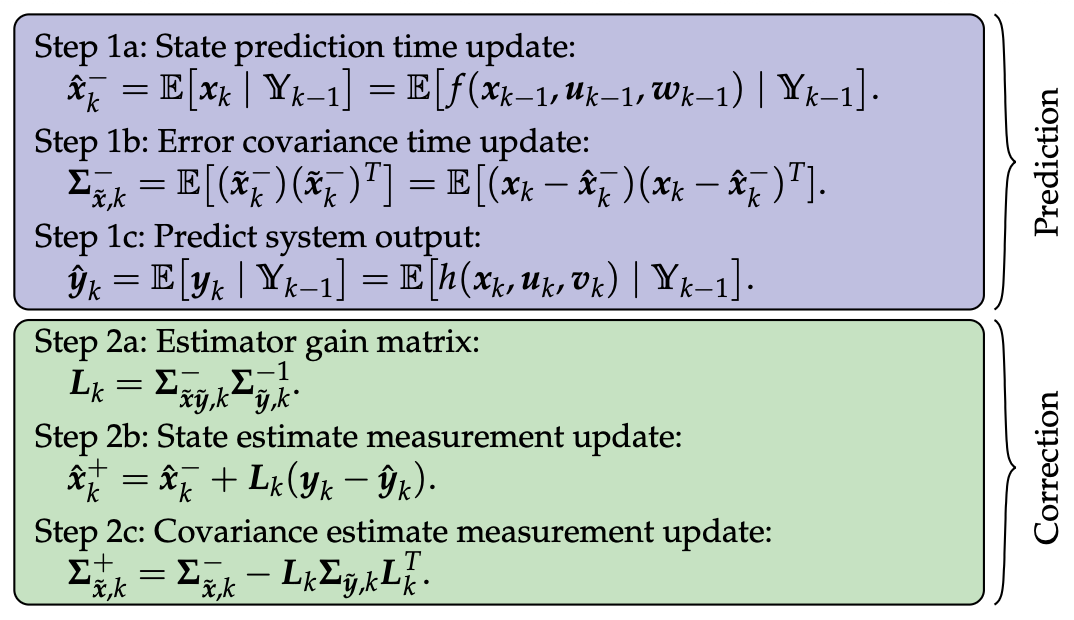
\includegraphics[width = 0.6\textwidth]{Images/StepsPredictionCorrection_KF.png}
%     \caption{Prediction and Correction steps in Kalman Filter algorithm~\cite{plett2015battery}.}
%     \label{img:KalmanFilterAlgorithmSteps_KF}
%   \end{figure}

\begin{figure}[htbp]
    \centering
  \begin{tikzpicture}[
    box/.style={
        draw, 
        rounded corners=4pt,
        inner sep=8pt, 
        text width=9cm, 
        font=\normalsize,
        line width=0.7pt
    },
    % Colors tailored to match the light purple/blue and light green
    predbox/.style={box, fill=blue!15},
    corrbox/.style={box, fill=green!17}
]

% Prediction Box
\node[predbox] (pred) {
    Step 1a: State prediction time update:\\
    \hspace*{1em} $\hat{\bm{x}}_k^- = \mathbb{E}[\bm{x}_k \mid \mathbb{Y}_{k-1}] = \mathbb{E}[f(\bm{x}_{k-1}, \bm{u}_{k-1}, \bm{w}_{k-1}) \mid \mathbb{Y}_{k-1}]$\\[0.5em]
    Step 1b: Error covariance time update:\\
    \hspace*{1em} $\bm{\Sigma}_{\tilde{\bm{x}},k}^- = \mathbb{E}[(\tilde{\bm{x}}_k^-)(\tilde{\bm{x}}_k^-)^T] = \mathbb{E}[(\bm{x}_k - \hat{\bm{x}}_k^-)(\bm{x}_k - \hat{\bm{x}}_k^-)^T]$\\[0.5em]
    Step 1c: Predict system output:\\
    \hspace*{1em} $\hat{\bm{y}}_k = \mathbb{E}[\bm{y}_k \mid \mathbb{Y}_{k-1}] = \mathbb{E}[h(\bm{x}_k, \bm{u}_k, \bm{v}_k) \mid \mathbb{Y}_{k-1}]$
};

% Correction Box
\node[corrbox, below=0.15cm of pred] (corr) {
    Step 2a: Estimator gain matrix:\\
    \hspace*{1em} $\bm{L}_k = \bm{\Sigma}_{\tilde{\bm{x}}\tilde{\bm{y}},k}^- \bm{\Sigma}_{\tilde{\bm{y}},k}^{-1}$\\[0.5em]
    Step 2b: State estimate measurement update:\\
    \hspace*{1em} $\hat{\bm{x}}_k^+ = \hat{\bm{x}}_k^- + \bm{L}_k(\bm{y}_k - \hat{\bm{y}}_k)$\\[0.5em]
    Step 2c: Covariance estimate measurement update:\\
    \hspace*{1em} $\bm{\Sigma}_{\tilde{\bm{x}},k}^+ = \bm{\Sigma}_{\tilde{\bm{x}},k}^- - \bm{L}_k \bm{\Sigma}_{\tilde{\bm{y}},k} \bm{L}_k^T$
};

% Braces
\draw[decorate,decoration={brace,amplitude=5pt},thick]
  ([xshift=3pt,yshift=-2pt]pred.north east) -- ([xshift=3pt,yshift=2pt]pred.south east)
  node[midway, xshift=15pt, rotate=-90, anchor=center] {Prediction};

  \draw[decorate,decoration={brace,amplitude=5pt},thick]
  ([xshift=3pt,yshift=-2pt]corr.north east) -- ([xshift=3pt,yshift=2pt]corr.south east)
  node[midway, xshift=15pt, rotate=-90, anchor=center] {Correction};

\end{tikzpicture}
\caption[Prediction and Correction steps in an Exteded Kalman Filter algorithm]
{Prediction and Correction steps in Kalman Filter algorithm~\cite{plett2015battery}.\protect\footnotemark}
\label{img:KalmanFilterAlgorithmSteps_KF}
\end{figure}
\footnotetext{During the preparation of this work,
the author used Gemini 3.5 to produce Figure~\ref{img:KalmanFilterAlgorithmSteps_KF}. After using this tool, the author reviewed and
edited the content as necessary, and she assumes full responsibility for the content of the publication.}


The Kalman Filter algorithm assumes a linear system or a nearly linear system. However, because the relationship between \acs{OCV} and \acs{SOC} 
is nonlinear, applying a linear filter introduces significant estimation inaccuracies. Consequently, different methodologies capable of 
addressing these nonlinear dynamics must be employed to ensure a more robust estimation.
\\
The nonlinear behaviour of the battery is shown in the following equations:
\begin{equation}
    x_k = f(x_{k-1}, u_{k-1}, w_{k-1}),
    \label{eq:nonlinearX}
\end{equation}

\begin{equation}
    y_k = h(x_k, u_k, v_k)
    \label{eq:nonlinearY}
\end{equation}
\\
\subsection{Extended Kalman Filter}

An extension of the Linear Kalman Filter is developed to address these nonlinearities, known as the Extended Kalman Filter (\acs{EKF}).
This method linearises the nonlinear system at each time step while following the same prediction and correction steps as the 
Kalman Filter (as shown in Figure~\ref{img:KalmanFilterAlgorithmSteps_EKF}). The linearisation is achieved through the computation of the 
Jacobian matrices, the partial derivatives of the nonlinear functions 
with respect to the relevant quantities being estimated. For the \acs{SOC} filter, these are the partial derivatives of the state and 
output equations with respect to the state vector $\hat{x}$, these matrices are shown as $\hat{A_k}$, $\hat{B_k}$, $\hat{C_k}$ and 
$\hat{D_k}$ in Section~\ref{SOCEKF}. For the \acs{SOH} filter, the Jacobians are taken with respect to the parameter vector $\theta$, 
and defined as $\hat{A_k^\theta}$, $\hat{B_k^\theta}$, $\hat{C_k^\theta}$, and $\hat{D_k^\theta}$ in Section~\ref{SOHEKF}.
By evaluating these matrices at the state estimate, the \acs{EKF} provides
a linear approximation of the system's behaviour around the operating point~\cite{plett2015battery}.

% \begin{figure}[H]
%     \centering
%     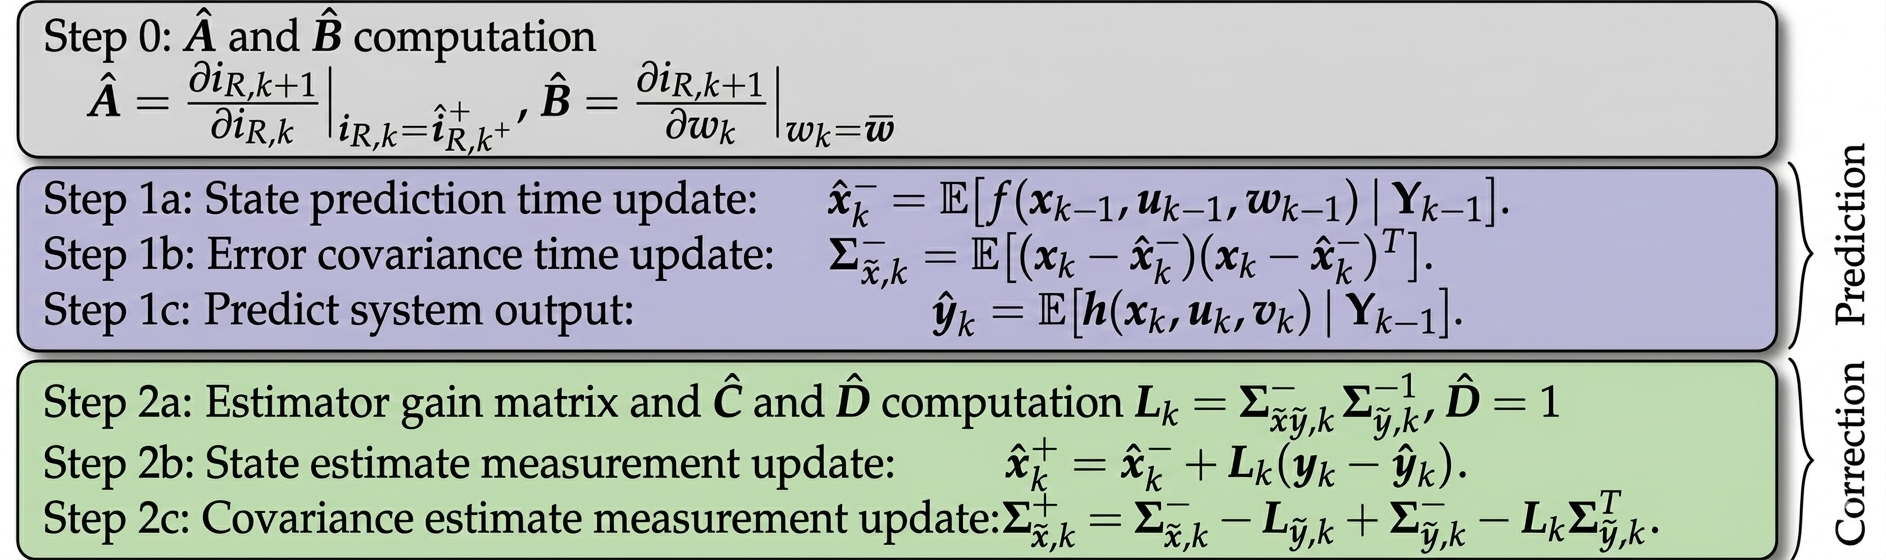
\includegraphics[width = 0.6\textwidth]{Images/StepsPredictionCorrection_EKF.png}
%     \caption{Prediction and Correction steps in an Extended Kalman Filter algorithm~\cite{plett2015battery}.}
%     \label{img:KalmanFilterAlgorithmSteps_EKF}
% \end{figure}

\begin{figure}[htbp]
    \centering
    \begin{tikzpicture}[
        box/.style={
            draw, 
            rounded corners=4pt,
            inner sep=8pt, 
            % Setting a fixed width ensures all three blocks match perfectly
            text width=10cm, 
            font=\small,
            line width=0.7pt
        },
        step0box/.style={box, fill=gray!20},
        predbox/.style={box, fill=blue!15},
        corrbox/.style={box, fill=green!17}
    ]

    % Step 0 Box (Gray)
    \node[step0box] (step0) {
        Step 0: $\hat{\bm{A}}$ and $\hat{\bm{B}}$ computation\\
        \vbox{\vspace*{0.3em}\centering $\hat{\bm{A}} = \left. \frac{\partial i_{R,k+1}}{\partial i_{R,k}} \right|_{i_{R,k}=\hat{i}_{R,k}^+}, 
        \quad \hat{\bm{B}} = \left. \frac{\partial i_{R,k+1}}{\partial \bm{w}_k} \right|_{\bm{w}_k=\bar{\bm{w}}}$}
    };

    % Prediction Box (Blue/Purple)
    \node[predbox, below=0.15cm of step0] (pred) {
        \begin{tabular}{@{}p{9cm} l@{}}
            Step 1a: State prediction time update: \\
            \hspace*{1em} $\hat{\bm{x}}_k^- = \mathbb{E}[f(\bm{x}_{k-1}, \bm{u}_{k-1}, \bm{w}_{k-1}) \mid \mathbb{Y}_{k-1}]$ \\[0.4em]
            Step 1b: Error covariance time update: \\
            \hspace*{1em} $\bm{\Sigma}_{\tilde{\bm{x}},k}^- = \mathbb{E}[(\bm{x}_k - \hat{\bm{x}}_k^-)(\bm{x}_k - \hat{\bm{x}}_k^-)^T]$ \\[0.4em]
            Step 1c: Predict system output: \\
            \hspace*{1em} $\hat{\bm{y}}_k = \mathbb{E}[h(\bm{x}_k, \bm{u}_k, \bm{v}_k) \mid \mathbb{Y}_{k-1}]$
        \end{tabular}
    };

    % Correction Box (Green)
    \node[corrbox, below=0.15cm of pred] (corr) {
        \begin{tabular}{@{}p{9cm} l@{}}
            Step 2a: Estimator gain matrix and $\hat{\bm{C}}$ and $\hat{\bm{D}}$ computation \\
            \hspace*{1em} $\bm{L}_k = \bm{\Sigma}_{\tilde{\bm{x}}\tilde{\bm{y}},k}^- \bm{\Sigma}_{\tilde{\bm{y}},k}^{-1}, \;\hat{\bm{D}} = 1$ \\[0.4em]
            Step 2b: State estimate measurement update: \\
            \hspace*{1em} $\hat{\bm{x}}_k^+ = \hat{\bm{x}}_k^- + \bm{L}_k(\bm{y}_k - \hat{\bm{y}}_k)$ \\[0.4em]
            Step 2c: Covariance estimate measurement update: \\
            \hspace*{1em} $\bm{\Sigma}_{\tilde{\bm{x}},k}^+ = \bm{\Sigma}_{\tilde{\bm{x}},k}^- - \bm{L}_k \bm{\Sigma}_{\tilde{\bm{y}},k} \bm{L}_k^T$
        \end{tabular}
    };

    % Braces pointing inward directly at their designated boxes
    \draw[decorate,decoration={brace,amplitude=5pt},thick]
      ([xshift=3pt,yshift=-2pt]pred.north east) -- ([xshift=3pt,yshift=2pt]pred.south east)
      node[midway, xshift=15pt, rotate=-90, anchor=center] {Prediction};

    \draw[decorate,decoration={brace,amplitude=5pt},thick]
      ([xshift=3pt,yshift=-2pt]corr.north east) -- ([xshift=3pt,yshift=2pt]corr.south east)
      node[midway, xshift=15pt, rotate=-90, anchor=center] {Correction};

    \end{tikzpicture}
    \caption[Prediction and Correction steps in an Exteded Kalman Filter algorithm]
    {Prediction and Correction steps in an Extended Kalman Filter algorithm~\cite{plett2015battery}.\protect\footnotemark}
    \label{img:KalmanFilterAlgorithmSteps_EKF}
\end{figure}
\footnotetext{During the preparation of this work,
the author used Gemini 3.5 to produce Figure~\ref{img:KalmanFilterAlgorithmSteps_EKF}. After using this tool, the author reviewed and
edited the content as necessary, and she assumes full responsibility for the content of the publication.}

\section{Dual Estimation Technique}\label{DualEstimator}

  In this work, the dual estimation approach is employed to perform the state and parameter estimation simultaneously. 
  Two separate \acs{EKF} algorithms are implemented in parallel, each operating on its respective estimation problem while 
  sharing state information at each time step. The \acs{SOC} estimator uses the updated \acs{ESR} and capacity values provided by 
  the \acs{SOH} filter, while the \acs{SOH} estimator incorporates the updated \acs{SOC} estimate.
  The interaction between the filters is shown in Figure~\ref{img:DualEstimationInteractionbetweenFilters}.

\begin{figure}[H]
    \centering
    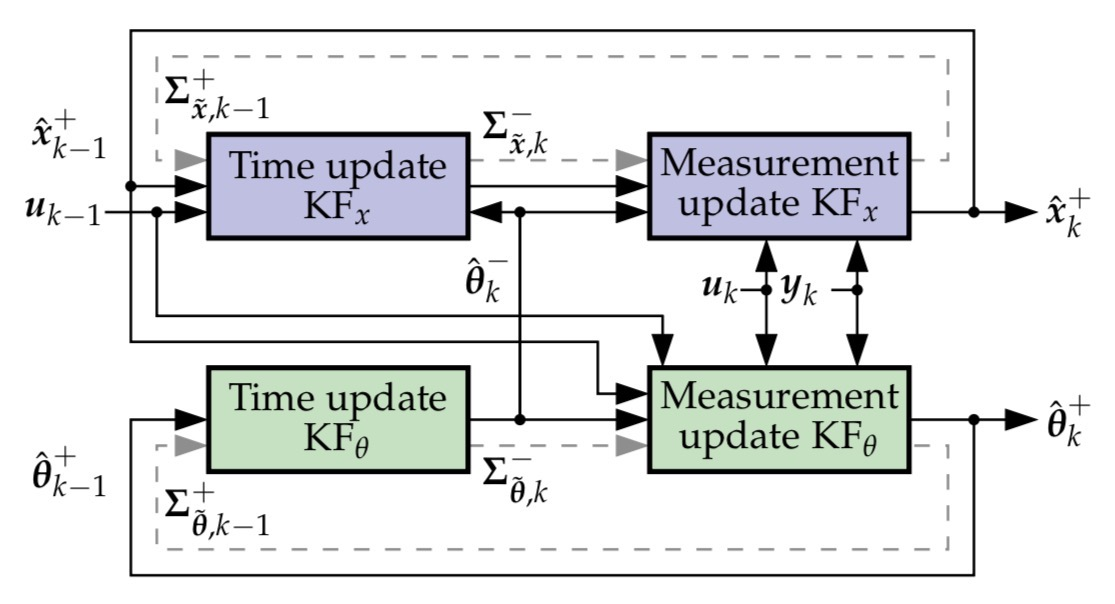
\includegraphics[width = 0.7\textwidth]{Images/InteractionsBetweenFiltersDualEstimation.jpg}
    \caption{Interaction between \acs{SOC} and \acs{SOH} Extended Kalman Filters using Dual Estimation~\cite{plett2015battery}.}
    \label{img:DualEstimationInteractionbetweenFilters}
\end{figure}

\section{EKF Implementation}\label{EKF}

The implementation of the algorithms described in Sections~\ref{SOCEKF},~\ref{SOHEKF}, and~\ref{dualEKF} and the steps shown in 
Section~\ref{EKFAlgorithm_Implementation} are translated into MATLAB code\footnote{During the preparation of this work,
the author used Claude Sonnet 4.6 to produce and improve sections of the MATLAB code. After using this tool, the author reviewed and 
edited the content as necessary, and she assumes full responsibility for the content of the publication.}, where the battery parameters 
and the \acs{OCV}/\acs{SOC} curve values obtained following the methodology described in Sections~\ref{Parameters} and~\ref{OCVSOC}, respectively,
are stored.

\subsection{EKF for SOC Estimation}\label{SOCEKF}

To implement the \acs{EKF} algorithm on a battery, the matrices $\hat{A_k}$, $\hat{B_k}$, $\hat{C_k}$ and $\hat{D_k}$ have to 
be determined based on the \acs{ECM} cell model.
These matrices represent the linearisation of the state equations~\eqref{eq:zESC},~\eqref{eq:iR1}, and~\eqref{eq:iR2} 
previously defined in 
Section~\ref{BatteryModel}.
\\
The state vector $\hat{x}$ comprises the currents flowing through the RC branches and the state of charge, 
which are the necessary variables to predict the terminal voltage according to equation~\eqref{eq:y_kESC}:
\begin{equation}
    \hat{x} = \begin{bmatrix}
    i_{R1}\\
    i_{R2}\\
    z
    \end{bmatrix}
\end{equation}

Assuming a Coulombic Efficiency of $\eta = 1$, the \acs{SOC} dynamics in equation~\eqref{eq:zESC} can be expressed as:
\\
\begin{equation}
    z_{k+1} = z_k - \frac{\Delta t}{Q}(i_k + w_k)
    \label{eq:zn1}
\end{equation}

To linearise the model, the partial derivatives of the state equations with respect to the state vector and the process noise 
have to be calculated. From equation~\eqref{eq:zn1}, the \acs{SOC}-related derivatives are:

\begin{equation}
    \left. \frac{\partial z_{k+1}}{\partial z_k} \right|_{z_k = \hat{z}_k^+} = 1
    \label{eq:zpartialderivativeA}
\end{equation}

\begin{equation}
    \left. \frac{\partial z_{k+1}}{\partial w_k} \right|_{w_k = \bar{w}} = - \frac{\Delta t}{Q}
    \label{eq:zpartialderivativeB}
\end{equation}

Similarly, the derivatives for the RC branch currents $i_{R1}$ and $i_{R2}$ are derived from equations~\eqref{eq:iR1}
and~\eqref{eq:iR2}, and are the following:

\begin{equation}
    \left. \frac{\partial i_{R1,k+1}}{\partial i_{R1,k}} \right|_{i_{R1,k} = \hat{i}_{R1,k}^+} = \tau_1
    \label{eq:ir1partialderivativeA}
\end{equation}

\begin{equation}
    \left. \frac{\partial i_{R2,k+1}}{\partial i_{R2,k}} \right|_{i_{R2,k} = \hat{i}_{R2,k}^+} = \tau_2
    \label{eq:ir2partialderivativeA}
\end{equation}

\begin{equation}
    \left. \frac{\partial i_{R1,k+1}}{\partial w_k} \right|_{w_k = \bar{w}} = 1-\tau_1
    \label{eq:ir1partialderivativeB}
\end{equation}

\begin{equation}
    \left. \frac{\partial i_{R2,k+1}}{\partial w_k} \right|_{w_k = \bar{w}} = 1-\tau_2
    \label{eq:ir2partialderivativeB}
\end{equation}

From previous equations~\eqref{eq:zpartialderivativeA},~\eqref{eq:ir1partialderivativeA}, and~\eqref{eq:ir2partialderivativeA} 
matrix $\hat{A}$ is constructed as follows:

\begin{equation}
    \hat{A}_k = \begin{bmatrix}
    \tau_1 & 0 & 0 \\
    0 & \tau_2 & 0 \\
    0 & 0 & 1
    \label{Amatrix}
    \end{bmatrix}
\end{equation}

Similarly, matrix $\hat{B}$ is assembled from equations~\eqref{eq:zpartialderivativeB},~\eqref{eq:ir1partialderivativeB}, 
and~\eqref{eq:ir2partialderivativeB}, resulting in:

\begin{equation}
    \hat{B}_k = \begin{bmatrix}
    1 - \tau_1 \\
    1 - \tau_2 \\
    -\frac{\Delta t}{Q}
    \label{Bmatrix}
    \end{bmatrix}
\end{equation}

The observation matrices $\hat{C}_k$ and $\hat{D}_k$ are obtained by differentiating the 
measurement equation~\eqref{eq:y_kESC} with respect to the state vector and measurement noise:

\begin{equation}
    \frac{\partial y_k}{\partial i_{R1}} = -R_1
    \label{eq:yKR1partialderivativeC}
\end{equation}

\begin{equation}
    \frac{\partial y_k}{\partial i_{R2}} = -R_2
    \label{eq:yKR2partialderivativeC}
\end{equation}

\begin{equation}
    \left. \frac{\partial y_k}{\partial z_k} \right|_{z_k = \hat{z}_k^-} = 
    \left. \frac{\partial OCV(z_k)}{\partial z_k} \right|_{z_k = \hat{z}_k^-}
    \label{eq:yKSOCpartialderivativeC}
\end{equation}

\begin{equation}
    \frac{\partial y_k}{\partial v_{k}} = 1
    \label{eq:yKvKpartialderivativeD}
\end{equation}

Thus, the resulting Jacobians from equations~\eqref{eq:yKR1partialderivativeC},~\eqref{eq:yKR2partialderivativeC}, 
and~\eqref{eq:yKSOCpartialderivativeC} form $\hat{C}$ as:
\begin{equation}
    \hat{C}_k = \begin{bmatrix}
    -R_1 & -R_2 & \frac{dOCV(z_k)}{dz}
    \label{Cmatrix}
    \end{bmatrix}
\end{equation}

And $\hat{D}$ from equation~\eqref{eq:yKvKpartialderivativeD} result in:

\begin{equation}
    \hat{D}_k = \begin{bmatrix}
    1
    \label{Dmatrix}
    \end{bmatrix}
\end{equation}

\subsection{EKF for SOH Estimation}\label{SOHEKF}
For \acs{SOH} estimation, the \acs{EKF} is formulated using the parameter vector defined in equation~\ref{eq:ThetaMatrix}, 
which contains the parameters selected for estimation, the equivalent series resistance $R_0$ and the cell capacity $Q$.
The dynamics of the parameters are modelled assuming that variations in $R_0$ and $Q$ occur slowly over time and exclusively due to 
perturbations, therefore a noise input is introduced. 
This white noise term ($r_{k-1}$) does not represent a physical quantity, rather, it is introduced to model the gradual 
variation of the cell parameters 
resulting from battery ageing. The dynamic is defined as follows:

\begin{equation}
    \theta_k = \theta_{k-1} + r_{k-1}
    \label{eq:ParametersEqwithNoise}
\end{equation}

where,

\begin{equation}
    \theta_k = \begin{bmatrix}
    R_0 \\
    Q
    \label{eq:ThetaMatrix}
    \end{bmatrix}
\end{equation}

The measurement function used for \acs{SOH} estimation is defined in equation~\ref{eq:nonlinearH} which derives from 
the output equation~\ref{eq:nonlinearY}, with the addition of the parameters in $\theta$ and the sensor noise and modelling error 
described in $e_k$.

\begin{equation}
    d_k = g(x_k, u_k, \theta, e_k)
    \label{eq:nonlinearH}
\end{equation}

For the \acs{SOH} filter, the state and input matrices ($\hat{A_k^\theta}$ and $\hat{B_k^\theta}$) are identity matrices due 
to the dynamics in equation~\ref{eq:ParametersEqwithNoise}. In contrast, the matrices $\hat{C_k^\theta}$ and $\hat{D_k^\theta}$ must be
calculated and are defined as follows:

% \begin{equation}
%     \left. \frac{\partial z_{k+1}}{\partial z_k} \right|_{z_k = \hat{z}_k^+} = 1
%     \label{eq:zpartialderivativeA}
% \end{equation}

\begin{equation}
    \left. \frac{dg(x_k, u_k, \theta, e_k)}{de_k} \right|_{e_k = \hat{e}_k^-} = \hat{D_k^\theta}
    \label{eq:DefinitionOfDtheta}
\end{equation}

\begin{equation}
    \left. \frac{dg(x_k, u_k, \theta, e_k)}{d\theta} \right|_{\theta = \hat{\theta}_k^-} = \hat{C_k^\theta} = 
    \frac{\partial g}{\partial \theta} + (\frac{\partial g}{\partial x_k})(\frac{d x_k}{d \theta})
    \label{eq:DefinitionOfCtheta}
\end{equation}

where, 
\begin{equation}
    g = OCV(z) -R_1 i_{R1} - R_2 i_{R2} - R_0 i_k
    \label{eq:nonlinearG}
\end{equation}

Further developing the terms for $\hat{C_k^\theta}$, taking into account equation~\ref{eq:nonlinearG},

\begin{equation}
    \frac{\partial g}{\partial R_0} = - i_k
\end{equation}

\begin{equation}
    \frac{\partial g}{\partial Q} = 0
\end{equation}

obtaining the first term of $\hat{C_k^\theta}$ as:

\begin{equation}
    \frac{\partial g}{\partial d\theta} = 
    \begin{bmatrix}
        - i_k \\
        0
    \end{bmatrix}
\end{equation}

For the second term in $\hat{C_k^\theta}$, the partial derivative of $g$ with respect to $x_k$ is computed as:

\begin{equation}
    \frac{\partial g}{\partial i_{R1}} = - R_1
\end{equation}

\begin{equation}
    \frac{\partial g}{\partial i_{R2}} = -R_2
\end{equation}

\begin{equation}
    \frac{\partial g}{\partial z} = \frac{dOCV}{dz}
\end{equation}

resulting in,

\begin{equation}
    \frac{\partial g}{\partial x_k} = 
    \begin{bmatrix}
        - R_1 \\
        - R_2 \\
        \frac{dOCV}{dz}
    \end{bmatrix}
\end{equation}

The final term required to compute $\hat{C_k^\theta}$ is recursive and obtained as,

\begin{equation}
    \frac{d x_k}{d\theta} = \frac{\partial f}{\partial \theta} + (\frac{\partial f}{\partial x_{k-1}})(\frac{d x_{k-1}}{d\theta})
    \label{LastTermofChatTotalDerivative}
\end{equation}

Taking the state equations~\ref{eq:iR1},~\ref{eq:iR2}, and~\ref{eq:zESC}, the corresponding partial derivatives 
with respect to $R_0$ and $Q$ can be calculated as:

\begin{equation}
    \frac{\partial i_{R1_k}}{\partial R_0} = 0
\end{equation}

\begin{equation}
    \frac{\partial i_{R2_k}}{\partial R_0} = 0
\end{equation}

\begin{equation}
    \frac{\partial z_k}{\partial R_0} = 0
\end{equation}

\begin{equation}
    \frac{\partial i_{R1_k}}{\partial \theta} = 0
\end{equation}

\begin{equation}
    \frac{\partial i_{R2_k}}{\partial \theta} = 0
\end{equation}

\begin{equation}
    \frac{\partial z_k}{\partial \theta} = \frac{\Delta t i_{k-1}}{Q^2}
\end{equation}

obtaining that,

\begin{equation}
    \frac{\partial f}{\partial \theta} = 
    \begin{bmatrix}
        0 && 0 \\
        0 && 0 \\
        0 && \frac{\Delta t i_{k-1}}{Q^2} \\
    \end{bmatrix}
\end{equation}

The final term~\ref{LastTermofChatTotalDerivative} captures the state evolution as a function of the parameters across time.
$\frac{\partial f}{\partial x_{k-1}}$ inside this equation is the Jacobian of the state transition function with respect to the
state vector evaluated at the previous estimate ($\hat{x}_{k-1}^+$), which is contained in the matrix $\hat{A}_{k-1}$ already obtained
in the \acs{SOC} estimation algorithm in Section~\ref{SOCEKF}.

Therefore substituting equation~\ref{LastTermofChatTotalDerivative} as,
\begin{equation}
    \frac{d x_k}{d\theta} = 
    \begin{bmatrix}
        0 && 0 \\
        0 && 0 \\
        0 && \frac{\Delta t i_{k-1}}{Q^2} \\
    \end{bmatrix} 
    + \hat{A}_{k-1}(\frac{d x_{k-1}}{d\theta})
    \label{LastTermofChatTotalDerivativewithAmatrix}
\end{equation}

This recursive term is initialised at $k=0$, since no prior information regarding the parameter is available at the beginning 
of the estimation process~\cite{plett2015battery}.

therefore $\hat{C_k^\theta}$ is,

\begin{equation}
    \hat{C_k^\theta} = 
    \begin{bmatrix}
        - i_k \\
        0
    \end{bmatrix} + 
    \begin{bmatrix}
        - R_1 \\
        - R_2 \\
        \frac{dOCV}{dz}
    \end{bmatrix}
    \begin{bmatrix}
        0 && 0 \\
        0 && 0 \\
        0 && \frac{\Delta t i_{k-1}}{Q^2} \\
    \end{bmatrix}
\end{equation}

For $\hat{D_k^\theta}$ the matrix is obtained as follows:

\begin{equation}
    \frac{\partial g}{\partial e_k} = 1
    \label{eq:DthetaPartial}
\end{equation}

Resulting in,

\begin{equation}
    \hat{D_k^\theta} = 1
    \label{eq:DthetaResult}
\end{equation}

\subsection{EKF Dual Implementation for SOC and SOH Estimation}\label{dualEKF}

In the dual estimation framework, both filters run simultaneously at each time step $k$, with the output of one serving as input to the other.
The \acs{SOC} filter requires the current parameter values $\theta_k^-$ to propagate the state and predict the terminal voltage accurately, 
since both the capacity $Q$ in the \acs{SOC} dynamics and the internal resistance $R_0$ in the output equation are elements of $\theta$.
To couple these two filters the equations~\ref{eq:nonlinearX} and~\ref{eq:nonlinearY} were modified as follows:

\begin{equation}
    x_k = f(x_{k-1}, u_{k-1}, \theta, w_{k-1})
    \label{eq:DualnonlinearX}
\end{equation}

\begin{equation}
    y_k = h(x_k, u_k, \theta, v_k)
    \label{eq:DualnonlinearY}
\end{equation}

Similarly, the \acs{SOH} filter requires an accurate estimate of the current state $\hat{x}_k^-$ to evaluate the output function~\ref{eq:nonlinearG}
and to propagate the recursive matrix. The information exchanged at each time step starts at the \acs{SOH} filter providing $\theta_k^-$ to the
\acs{SOC} filter before the state propagation step. The \acs{SOC} filter provides $\hat{x}_k^-$, $\hat{x}_k^+$ and the Kalman gain $L$ to the \acs{SOH} filter,
which uses them to evaluate the function shown in equation~\ref{eq:nonlinearG} to compute $\hat{C_k^\theta}$, and to update its algorithm.
The complete execution order of the coupled algorithm is detailed in the following Section~\ref{EKFAlgorithm_Implementation}.

\subsection{Recursive Algorithm}\label{EKFAlgorithm_Implementation}

Once the Jacobian matrices are defined, as previously shown in sections~\ref{SOCEKF} and~\ref{SOHEKF}, 
they have to be integrated into their corresponding Kalman Filter recursive algorithm and updated at each time step. 
The \acs{EKF} algorithm goes through a recursive three-stage process which consists of updating the $\hat{A}_{k-1}$ and $\hat{B}_{k-1}$ 
matrices, then the time update (prediction), and measurement update (correction).

\begin{itemize}
    \item \textbf{Step 0}
        \begin{itemize}
            \item[\(\circ\)] \textbf{\acs{SOC}} - Update $\hat{A}_{k-1}$ and $\hat{B}_{k-1}$ (matrices shown in~\eqref{Amatrix} and~\eqref{Bmatrix})
        \end{itemize}
    \item \textbf{Step 1a} - Parameter Prediction Time Update
        \begin{itemize}
            \item[\(\circ\)] \textbf{\acs{SOC}} - Propagate the state estimate forward using the nonlinear system dynamics and the measured current $i_k$,
            and update current $Q$ value stored in $\theta$ vector.
                \begin{equation}
                    \hat{x}_k^- = f(\hat{x}_{k-1}^+, u_{k-1}, w_{k-1}, \theta_k^-)
                \end{equation}
                \item[\(\circ\)] \textbf{\acs{SOH}} - Update the recursive sensitivity matrix $\frac{dx_k}{d\theta}$ by applying the updated 
                $\hat{A}_{k-1}$ and $\frac{\partial f}{\partial \theta}$ values computed in Step 0.
            \end{itemize}
    \item \textbf{Step 1b} - Error Covariance Time Update
        \begin{itemize}
            \item[\(\circ\)] \textbf{\acs{SOC}} - Project the uncertainty forward, accounting for the process noise covariance $\Sigma_w$.
            \begin{equation}
                \Sigma_{x,k}^- = \hat{A}_{k-1} \Sigma_{x,k-1}^+ \hat{A}_{k-1}^T + \hat{B}_{k-1} \Sigma_w \hat{B}_{k-1}^T
            \end{equation}
            \item[\(\circ\)] \textbf{\acs{SOH}} - Predict the parameter uncertainty forward, accounting for the process noise covariance $\Sigma_{r,k-1}$
            \begin{equation}
                \Sigma_{\theta,k}^- = \Sigma_{\theta,k-1}^+ + \Sigma_{r,k-1}
            \end{equation}
        \end{itemize}
    \item \textbf{Step 1c} - Output Prediction
        \begin{itemize}
            \item[\(\circ\)] \textbf{\acs{SOC}} - Calculate the predicted terminal voltage.
            \begin{equation}
                \hat{y}_k = h(\hat{x}_k^-, i_k, \theta_k^-)
            \end{equation}
            \item[\(\circ\)] \textbf{\acs{SOH}} - Predicted output is evaluated using the prior state estimate $\hat{x}_k^-$ 
            from the \acs{SOC} filter and the prior parameter estimate $\theta_k^-$.
            \begin{equation}
                \hat{d}_k = g(\hat{x}_k^-, u_k, \theta_k^-) = OCV(z_k^-) - R_1 i_{R1,k}^- - R_2 i_{R2,k}^- - R_0 i_k
            \end{equation}
        \end{itemize}
    \item \textbf{Step 2a} - Estimator Gain Matrix
        \begin{itemize}
            \item[\(\circ\)] \textbf{\acs{SOC}} - Update $\hat{C}_{k-1}$ and $\hat{D}_{k-1}$ matrices shown in~\eqref{Cmatrix} and~\eqref{Dmatrix} 
            respectively and calculate the optimal gain $L_k$ by weighing the model uncertainty against the measurement noise 
            covariance $\Sigma_v$.
            \begin{equation}
                \Sigma_{y,k} =  \hat{C}_k \Sigma_{x,k}^- \hat{C}_k^T + \hat{D}_k \Sigma_v \hat{D}_k^T
            \end{equation}
            \begin{equation}
                L_k = \Sigma_{x,k}^- \hat{C}_k^T (\Sigma_{y,k})^{-1}
            \end{equation}
            \item[\(\circ\)] \textbf{\acs{SOH}} - Update $\hat{C}_{k-1}^\theta$ and $\hat{D}_{k-1}^\theta$ by deriving using chain rule
            as shown in Section~\ref{SOHEKF} and obtain covariance and Kalman filter gain.
            \begin{equation}
                \Sigma_{d,k} =  \hat{C}_k^\theta \Sigma_{\theta,k}^- (\hat{C}_k^\theta)^T + \hat{D}_k^\theta \Sigma_e (\hat{D}_k)^T
            \end{equation}
            \begin{equation}
                L_k^\theta = \Sigma_{\theta,k}^- (\hat{C}_k^\theta)^T (\Sigma_{d,k})^{-1}
            \end{equation}
        \end{itemize}
    \item \textbf{Step 2b} - Parameter Estimate Measurement Update
        \begin{itemize}
            \item[\(\circ\)] \textbf{\acs{SOC}} - Correct the predicted state using the residual between the measured voltage $v_k$ and the predicted voltage $\hat{y}_k$.
            \begin{equation}
                r = y_k - \hat{y}_k
            \end{equation}
            \begin{equation}
                \hat{x}_k^+ = \hat{x}_k^- + L_k r
            \end{equation}
            \item[\(\circ\)] \textbf{\acs{SOH}} - Compute a posteriori $R_0$ and $Q$ parameters stored in vector $\theta$ by obtaining the output prediction error $r$.
            \begin{equation}
                r = d_k - \hat{d}_k
            \end{equation}
            \begin{equation}
                \hat{\theta}_k^+ = \hat{\theta}_k^- + L_k^\theta r
            \end{equation}
        \end{itemize}
    \item \textbf{Step 2c} - Error Covariance Measurement Update
        \begin{itemize}
            \item[\(\circ\)] \textbf{\acs{SOC}} - Update the covariance matrix to reflect the reduction in uncertainty after incorporating the measurement.
                \begin{equation}
                    \Sigma_{x,k}^+ = \Sigma_{x,k}^- - L_k \Sigma_{y,k} L_k^T
                \end{equation}
                \item[\(\circ\)] \textbf{\acs{SOH}} - Update covariance $\Sigma_{\theta,k}^+$.
                \begin{equation}
                    \Sigma_{\theta,k}^+ = \Sigma_{\theta,k}^- - L_k^\theta \Sigma_{d,k} (L_k^\theta)^T
                \end{equation}
        \end{itemize}
\end{itemize}

% Step 1a xhat⁻ = f(xhat⁺, i_k) which Propagates the state forward using prior current I
% Step 1b Σ⁻ = Ahat·Σ⁺·Ahat' + Bhat·SigmaW·Bhat' for Growing the uncertainty (model uncertainty increases between measurements)
% Step 1c yhat = h(xhat⁻, i_k) Predicting what the voltage should be
% Step 2a L = Σ⁻·Chat' / (Chat·Σ⁻·Chat' + SigmaV) for Kalman gain: how much to trust voltage vs model
% Step 2b xhat⁺ = xhat⁻ + L·(vk - yhat) Correcting state using measurement residual
% Step 2c Σ⁺ = Σ⁻ - L·SigmaY·L' for Shrink uncertainty after using measurement

% \section{System Integration?}\label{SystInt}
% Section 5 — System Integration (if relevant)
% How this fits within the eRacing BMS. Inputs available in real time (current, cell voltages, temperature). 
% Master-Slave architecture constraints. Sampling rate considerations.

% Section 6 — Algorithm Extensions
% Write this section in future tense or conditional framing:
% "Depending on the accuracy achieved by the base EKF implementation, two extensions are considered: (a) 
% the Unscented Kalman Filter, which avoids linearisation by propagating sigma points through the nonlinear model; 
% (b) joint SOC/SOH estimation via a Dual EKF operating on two timescales. The selection between these approaches will 
% be guided by the validation results presented in Chapter X."
% This section can be one page now and expand later into your actual implementation.